
%%%%%%%%%%%%%%%%%%%%%%%%%%%%%%%%%%%%%%%%%
% University/School Laboratory Report
% LaTeX Template
% Version 3.1 (25/3/14)
%
% This template has been downloaded from:
% http://www.LaTeXTemplates.com
%
% Original author:
% Linux and Unix Users Group at Virginia Tech Wiki 
% (https://vtluug.org/wiki/Example_LaTeX_chem_lab_report)
%
% License:
% CC BY-NC-SA 3.0 (http://creativecommons.org/licenses/by-nc-sa/3.0/)
%
%%%%%%%%%%%%%%%%%%%%%%%%%%%%%%%%%%%%%%%%%

%----------------------------------------------------------------------------------------
%	PACKAGES AND DOCUMENT CONFIGURATIONS
%----------------------------------------------------------------------------------------

\documentclass{article}
\usepackage[margin=1.25in]{geometry}
\usepackage{hyperref}
\usepackage[version=3]{mhchem} % Package for chemical equation typesetting
\usepackage{siunitx} % Provides the \SI{}{} and \si{} command for typesetting SI units
\usepackage{graphicx} % Required for the inclusion of images
\usepackage{natbib} % Required to change bibliography style to APA
\usepackage{amsmath} % Required for some math elements 

\setlength\parindent{1em} % Removes all indentation from paragraphs
\setlength{\parskip}{1em}
\renewcommand{\labelenumi}{\alph{enumi}.} % Make numbering in the enumerate environment by letter rather than number (e.g. section 6)

%\usepackage{times} % Uncomment to use the Times New Roman font

%----------------------------------------------------------------------------------------
%	DOCUMENT INFORMATION
%----------------------------------------------------------------------------------------

\title{Weekly Catchup} % Title

\author{Weixiong Zheng} % Author name

\date{\today} % Date for the report

\begin{document}

\maketitle % Insert the title, author and date
% If you wish to include an abstract, uncomment the lines below
% \begin{abstract}
% Abstract text
% \end{abstract}

%----------------------------------------------------------------------------------------
%	SECTION 0
%----------------------------------------------------------------------------------------
\section{Updates on previous goals}
Previous goals include redesigning BARTDriver and help Marissa on debugging.

%----------------------------------------------------------------------------------------
%	SECTION 1
%----------------------------------------------------------------------------------------
\section{Progress up to now}
The BARTDriver re-implementation was slowed down because of the stuck PR reviewing as Josh
leaving for the new baby. Meanwhile, some wonderful things came during the spring recess.

The biggest progress is that I found out the error claimed as initial cell error. It was
a serendipity that I found out doing calculations using even parity equation without
reflective boundary condition imposed actually have consistent results however many processors are used. Figure 1\ is an example of 384-cell domain decomposed to seven processors along with the corresponding global scalar flux. Figure 2\ demonstrates the efficacy of distributing solutions with \[\mathrm{n\_cell}\%\mathrm{n\_proc}\neq0\].

\begin{figure}
	\centering
	
\includegraphics[width=0.7\textwidth]{solu.png}
	\caption{Demo of calculation on 7 processors for 384 cells.}
\end{figure}
\begin{figure}
	\centering
	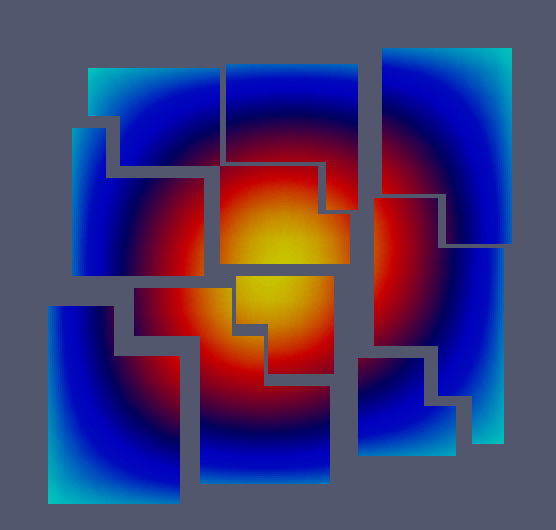
\includegraphics[width=.6\textwidth]{decomp-solu.png}
	\caption{Solutions distributed on decomposed subdomains.}
\end{figure}

The other accomplishment is that a trial has been successfully done in producing fuel 
pin using deal.II functions. Before, it was claimed that doing fuel-pin resolved calculations need third-party libraries to generate the mesh. Now, it is hopeful that
with reasonable amount of work pin-resolved mesh can be generated just as structured mesh in BART. Figure 3 is a demo of a bunch of \boxed{C5G7} pins. This functionality will appear soon in BART.

\begin{figure}
	\centering
	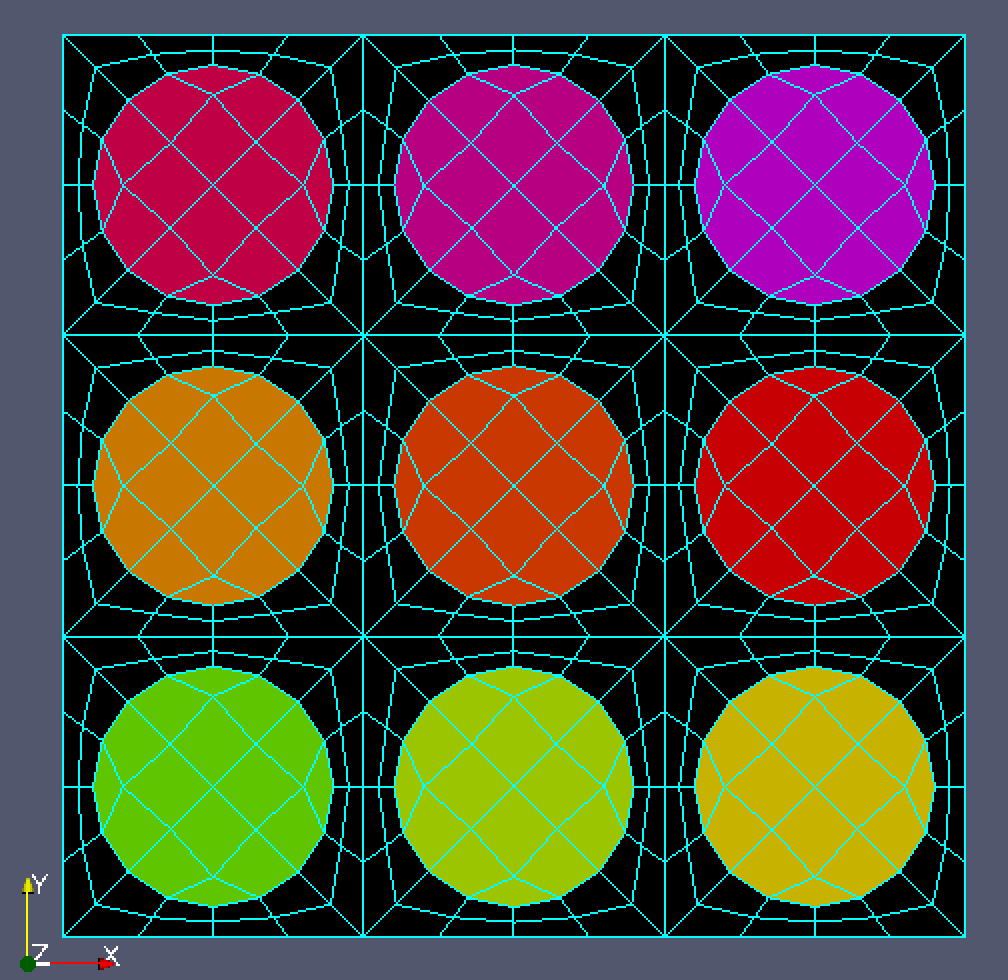
\includegraphics[width=0.8\textwidth]{rods}
	\caption{Fuel pins}
\end{figure}
%----------------------------------------------------------------------------------------
%	SECTION 2
%----------------------------------------------------------------------------------------
\section{Things you need from Rachel}


%----------------------------------------------------------------------------------------
%	SECTION 3
%----------------------------------------------------------------------------------------
\section{Goals/Things will be going on}
It is a special time that Josh will not be able to review the code. I will keep on going however
to restart the BART with:
\begin{itemize}
	\item new/more reasonable designs of classes/namespaces during restart.
	\item adding unstructured mesh functionality.
	\item see if I can help Marissa get through the bugs.
\end{itemize}

%----------------------------------------------------------------------------------------
%	SECTION 4
%----------------------------------------------------------------------------------------
%\section{Links to any related materials}



%----------------------------------------------------------------------------------------
%	BIBLIOGRAPHY
%----------------------------------------------------------------------------------------

%\bibliographystyle{apalike}
%
%\bibliography{sample}

%----------------------------------------------------------------------------------------


\end{document}